\documentclass[12pt,a4paper]{article}
% 如果需要中文支持，推荐使用xeCJK + 字体设置
% \usepackage{xeCJK}
% \setCJKmainfont{SimSun}  % 示例：宋体，可根据系统字体情况更换
\usepackage{ctex}
\setlength{\parindent}{2em}
\setlength{\parskip}{0pt} % 确保段落之间没有额外的空行间距


\usepackage{amsmath}      % 数学公式（如有需要）
\usepackage{graphicx}     % 插图
\usepackage{geometry}     % 调整页边距
\usepackage{fancyhdr}     % 自定义页眉页脚
\usepackage{indentfirst}  % 中文首行缩进
\usepackage{calc}         % 允许做长度运算(测量文字宽度等)
\usepackage{titlesec}
\usepackage{booktabs} % 解决 \midrule 和 \bottomrule 报错
\usepackage{enumitem} % 支持自定义列表格式
\usepackage{float}    % 支持强制浮动位置
\usepackage{siunitx}
\usepackage{wrapfig}

% 设置 \section 级标题为：加粗、大字号（如 \Large）
\titleformat{\section}
	{\bfseries\large}    % 标题自身的格式
	{\thesection}        % 标题编号的显示方式
	{1em}                % 编号与标题文字之间的间距
	{}                   % 在标题文字前后可插入额外代码，此处为空
	
% 设置 \subsection 级标题为：加粗、中等字号（如 \normalsize）
\titleformat{\subsection}
	{\bfseries\normalsize}
	{\thesubsection}
	{1em}
{}

% 页面设置（可根据需要微调）
\geometry{
	left=2cm,
	right=2cm,
	top=1cm,
	bottom=1.5cm
}

% 不需要过大的行距，使用较接近单倍行距的设置
\renewcommand{\baselinestretch}{1.2}

% 仅在页脚居中显示页码，页眉保持为空
\pagestyle{fancy}
\fancyhf{}  % 清空默认的页眉页脚
\fancyfoot[C]{\thepage}
\renewcommand{\headrulewidth}{0pt}
\renewcommand{\footrulewidth}{0pt}

% 首行缩进2字符(中文习惯)
% \setlength{\parindent}{0pt}
\setlength{\leftskip}{2em}
\setlength{\parindent}{2em}

\begin{document}
	%-------------------------------------------------------
	% 1 并排两个minipage：左标题、右校徽
	%   - 0.65\textwidth + 0.35\textwidth = \textwidth
	%   - 如果校徽过大或过小，可改宽度，如 0.25\textwidth、0.3\textwidth 等
	%   - 如果想让标题更大，可将 \Huge 改成 \huge 或 \LARGE
	%-------------------------------------------------------
	\noindent
	\hspace{-2em}
	\begin{minipage}[c]{0.65\textwidth}
		\raggedright
		{\fontsize{35pt}{55pt}\selectfont 物理实验报告}
	\end{minipage}
	\begin{minipage}[c]{0.35\textwidth}
		\raggedleft
		% 强制把校徽拉大到 0.35\textwidth 宽度 (高度自动匹配)
		% 若想指定高度,可用 "height=3cm" 等. 二选一即可.
		
\includegraphics[width=\linewidth, trim={20cm 20cm 20cm 20cm}, clip]{university_logo.png}
	\end{minipage}

	\vspace{-1em}
	

	%下方画两条分割线，并在两线之间写学号、姓名、日期、时间
	
	\hrule
	\vspace{0.6em}
	\noindent
	\begin{tabular}{l l l l}
    学号：12411434 & 姓名：{郑宇轩} &
    日期：2025.12.01 & 时间：周一下午
	\end{tabular}
	\vspace{0.4em}
	\par
	\hrule

	
	\section*{\textbf{一. 实验名称：光电效应法测普朗克常量}}
	
	\section*{\textbf{二. 实验目的}}
	\begin{enumerate}
		\item 了解光电效应的基本规律,用光电效应方法测量普朗克常量 $h$、材料的逸出功 $A$ 和红限值 $\nu_0$。

	\end{enumerate}

	\section*{\textbf{{三. 实验原理}}}

	\begin{enumerate}

	\item \textbf{光电效应原理}
	
	光电效应是指光照射在物体上，使电子获得能量并逸出物体表面的现象，逸出的电子称为光电子。根据爱因斯坦提出的光子假设，光子能量为 $\varepsilon = h\nu$，光电子吸收光子能量后，部分消耗用于克服逸出功 $A$，剩余部分转化为动能，遵循能量守恒公式
	\begin{equation}
	h\nu = \frac{1}{2}mv^2 + A
	\end{equation}
	即为爱因斯坦光电效应方程，其中 $h$ 为普朗克常数，$A$为材料的逸出功。由此可知，光电子初动能与入射光频率 $\nu$ 呈线性关系，而与入射光强度无关。光电流随加速电势差 \( U \) 增大而增加，并在饱和值 \( I_h \) 处趋于稳定，其大小与光强成正比而与频率无关。当 \( U \) 为负值时，光电流迅速减小，达到遏止电势差时降为零。此时，光电子的最大动能与电势能相等，故
	\begin{equation}
		eU_a = h \nu - A
	\end{equation}
	其中 \( U_a \) 为遏止电势差，\( e \) 为电子电荷量。

	\item \textbf{光电效应实验}
	
	光电效应实验原理如下图所示，其中 S 为真空光电管。当无光照射阴极时，电路中无电流流过；当短波单色光照射阴极 K 时，会产生光电流，其大小随加速电势差 $U$ 变化，形成特定的伏安特性曲线。
	\begin{figure}[H]
		\centering
		
\includegraphics[width=0.4\textwidth]{1.jpg}
		
\includegraphics[width=0.4\textwidth]{2.jpg}
		\caption{光电效应原理图}
		\label{fig:chart1}
	\end{figure}

	实验指出，存在红限频率 $\nu_0$，当光的频率 $\nu < \nu_0$ 时，不论用多强的光照射到物质都不会产生光电效应。根据公式$\frac{1}{2}mv^2 = eU_A$，可以得到 $\nu_0 = \frac{A}{h}$，其中 $A$ 为逸出功。遏止电压公式也可写作如下形式：
		
	\begin{equation}
		U_a = \dfrac{h}e \nu - \dfrac{A}e
	\end{equation}
	
	实验得到伏安特性曲线后，测量不同频率单色光对应的遏止电势差 $U_A$，作出 $U_A - \nu$ 图像，线性拟合求出普朗克常数 $h$ 和逸出功 $A$，进而计算得到 $\nu_0$。

	
	\end{enumerate}
	
	\section*{\textbf{{四. 实验仪器}}}
	光电管、滤波片、汞灯、微电流计、直流电源

	\section*{\textbf{{五. 实验内容}}}

	按照图1方式接线，分别在波长为 577nm、546nm、436nm、405nm、365nm 五种单色光下测量光电管的伏安特性曲线。在每种单色光下，外加电压调整至 \(-2V \sim 0V\) 范围内，每隔 0.1V 记录一个数据点，至少记录20个数据点，根据所得曲线确定对应的遏止电压 $U_a$。线性拟合 $U_a - \nu$ 曲线，求得普朗克常数 $h$、逸出功 $A$ 和红限频率 $\nu_0$。
	
	\section*{\textbf{{六. 数据记录}}}
	
	原始测量数据见附表 1。

	\section*{\textbf{{七. 数据处理}}}

	\begin{enumerate}

	\item \textbf{不同波长光电管伏安特性曲线}
	
	\begin{figure}[H]
		\centering
		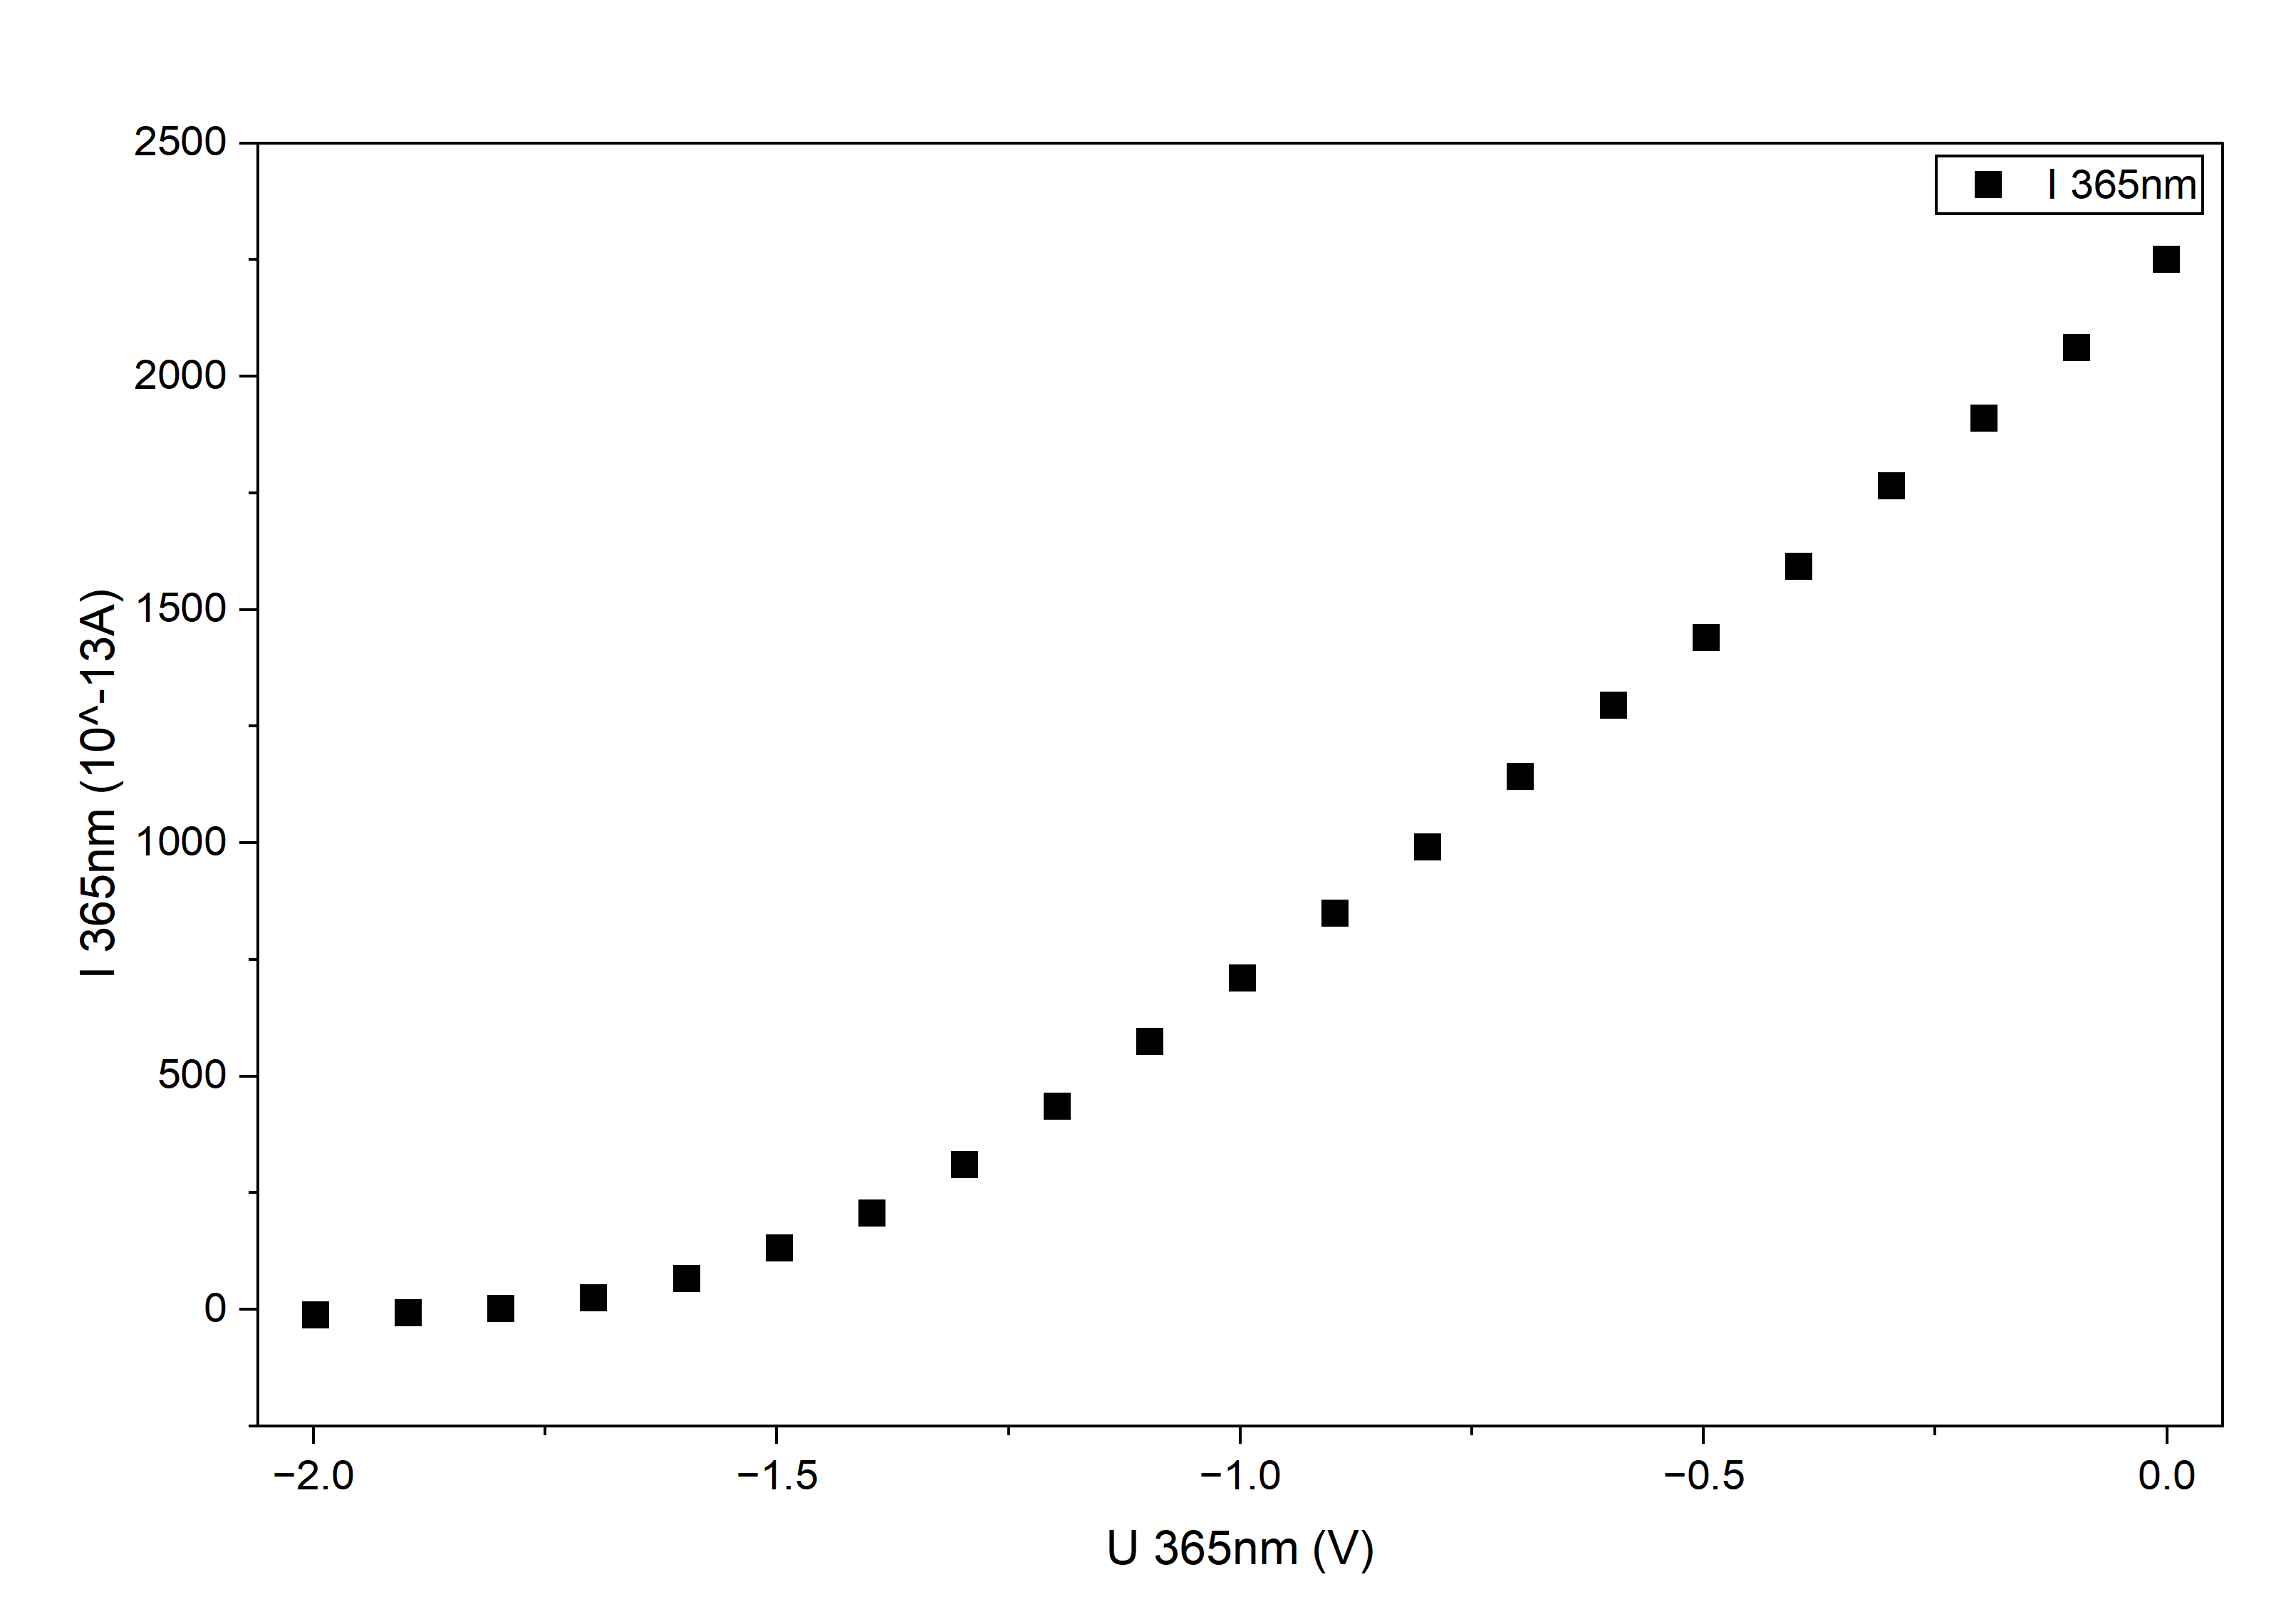
\includegraphics[width=0.9\textwidth]{365.png}
		\caption{365nm 波长光电管伏安特性曲线}
		\label{fig:365nm}
	\end{figure}
	\begin{figure}[H]
		\centering
		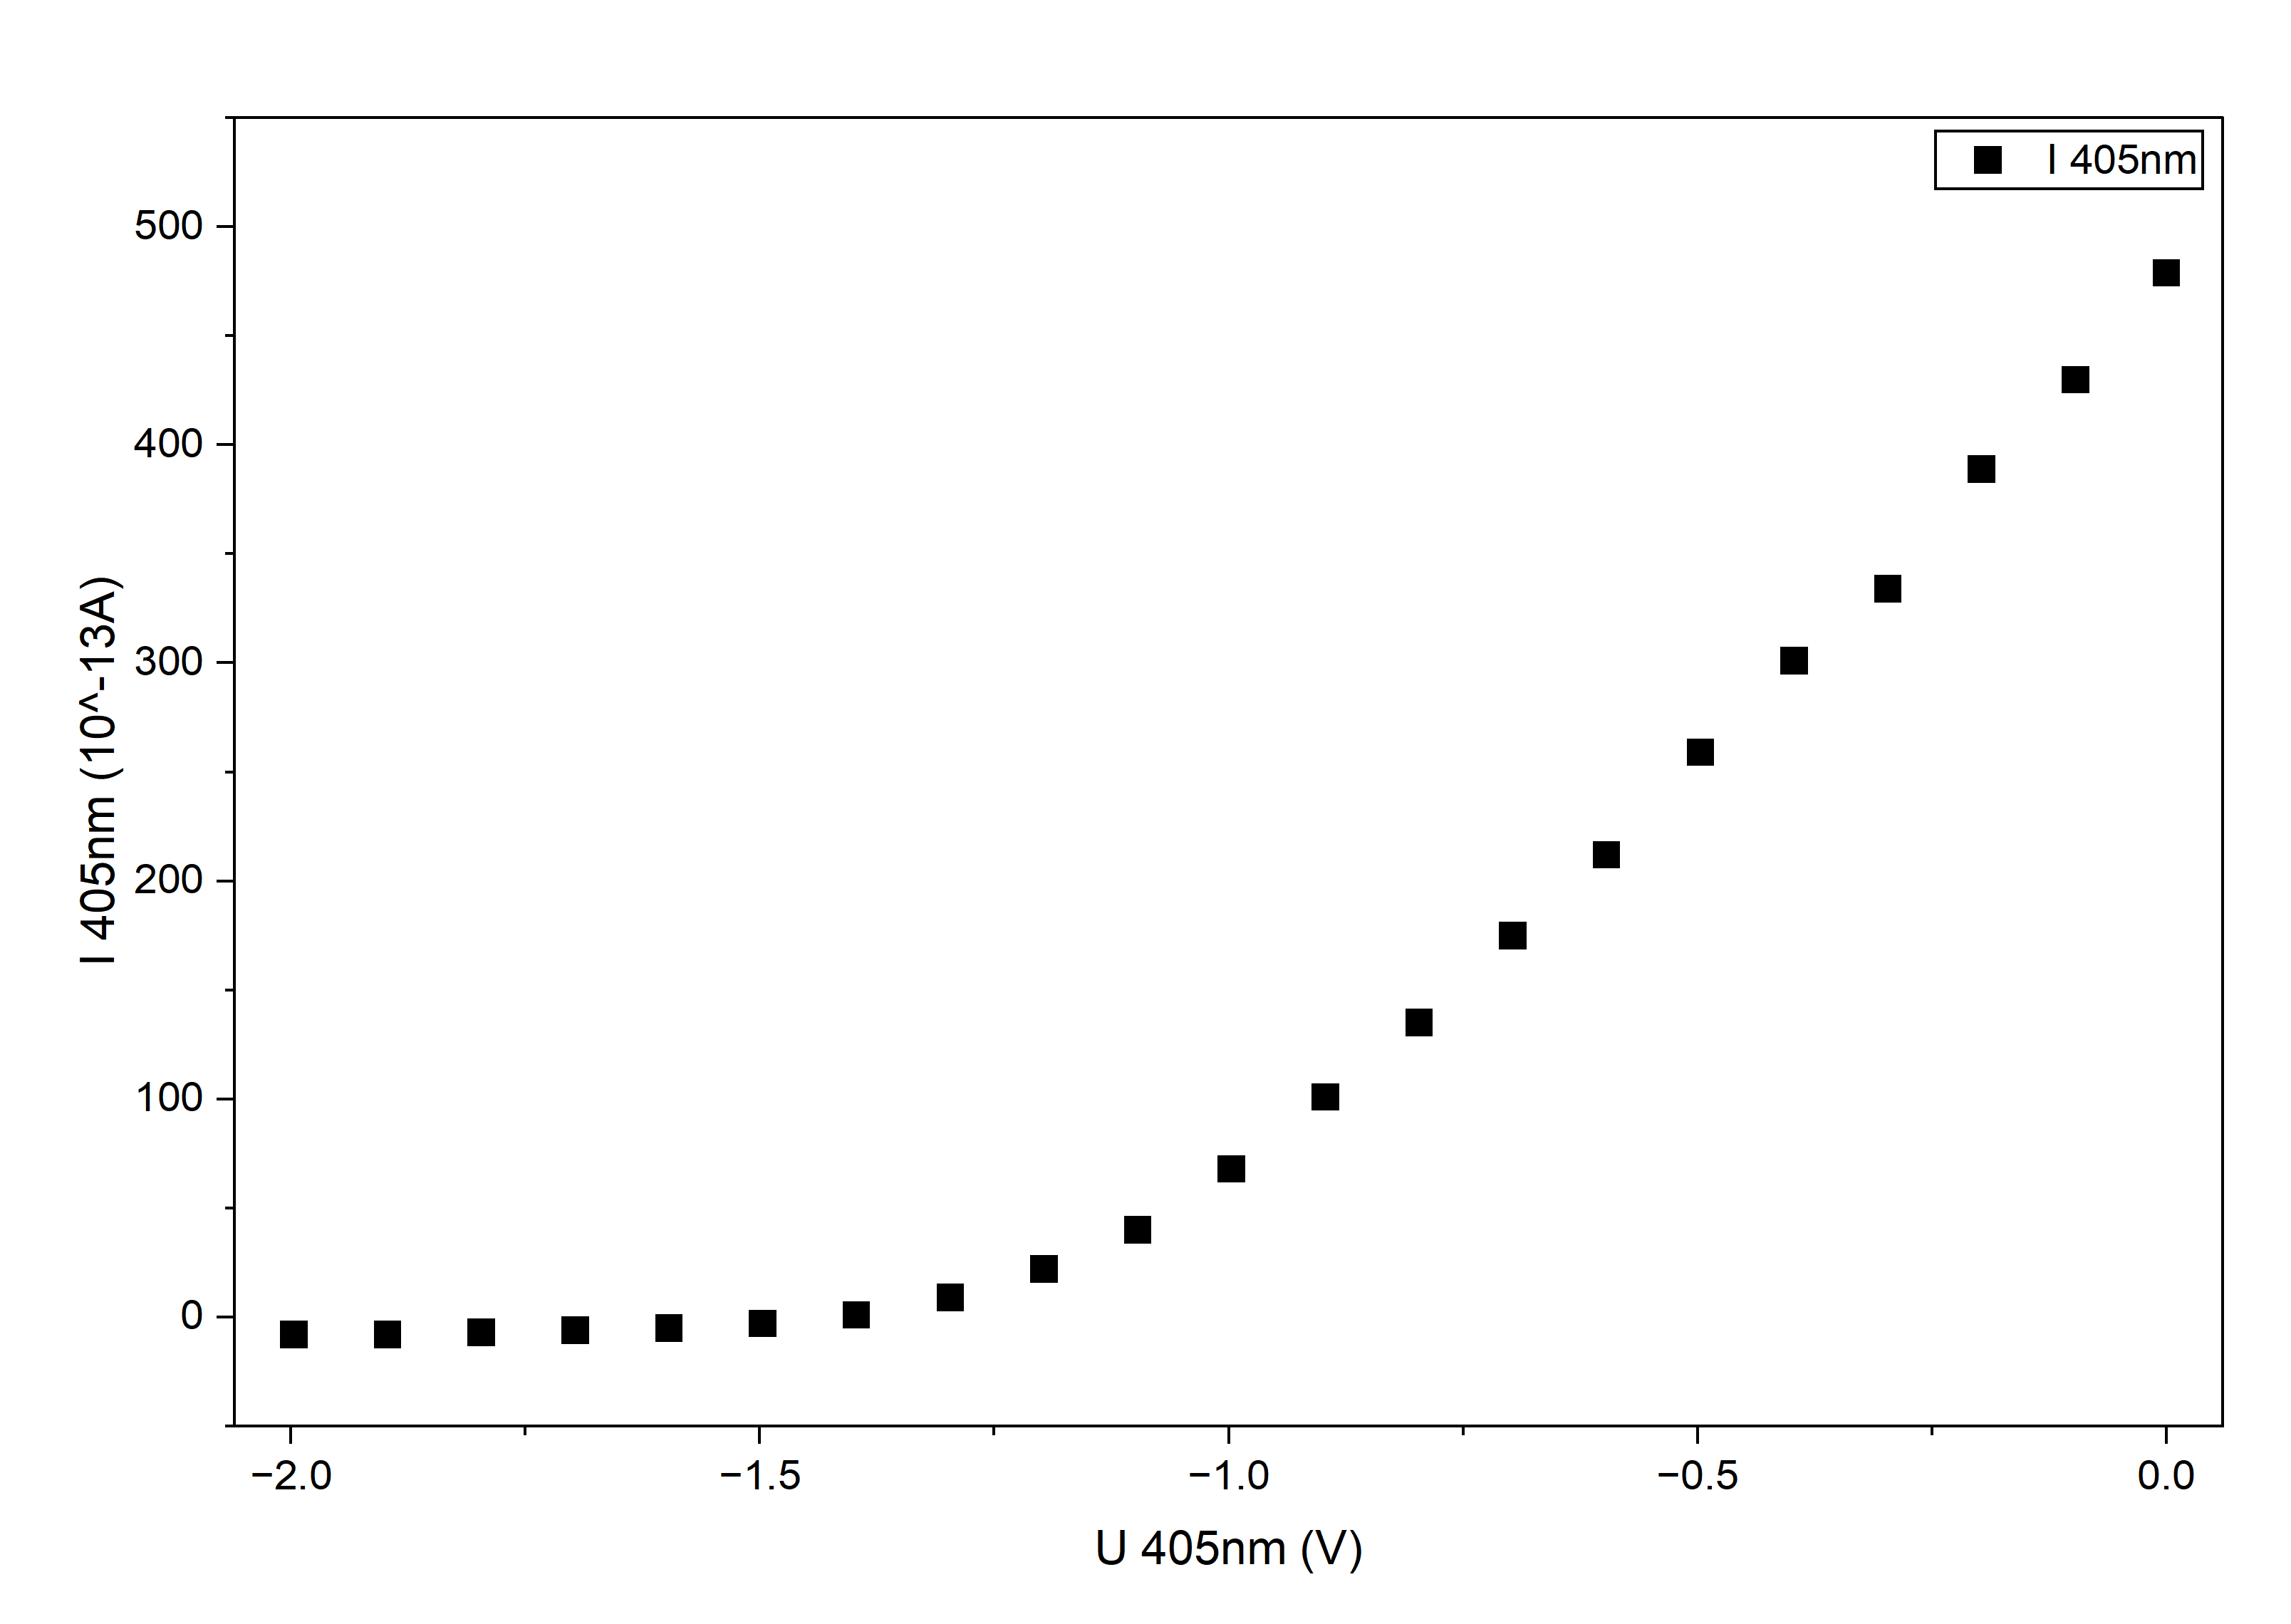
\includegraphics[width=0.9\textwidth]{405.png}
		\caption{405nm 波长光电管伏安特性曲线}
		\label{fig:405nm}
	\end{figure}\begin{figure}[H]
		\centering
		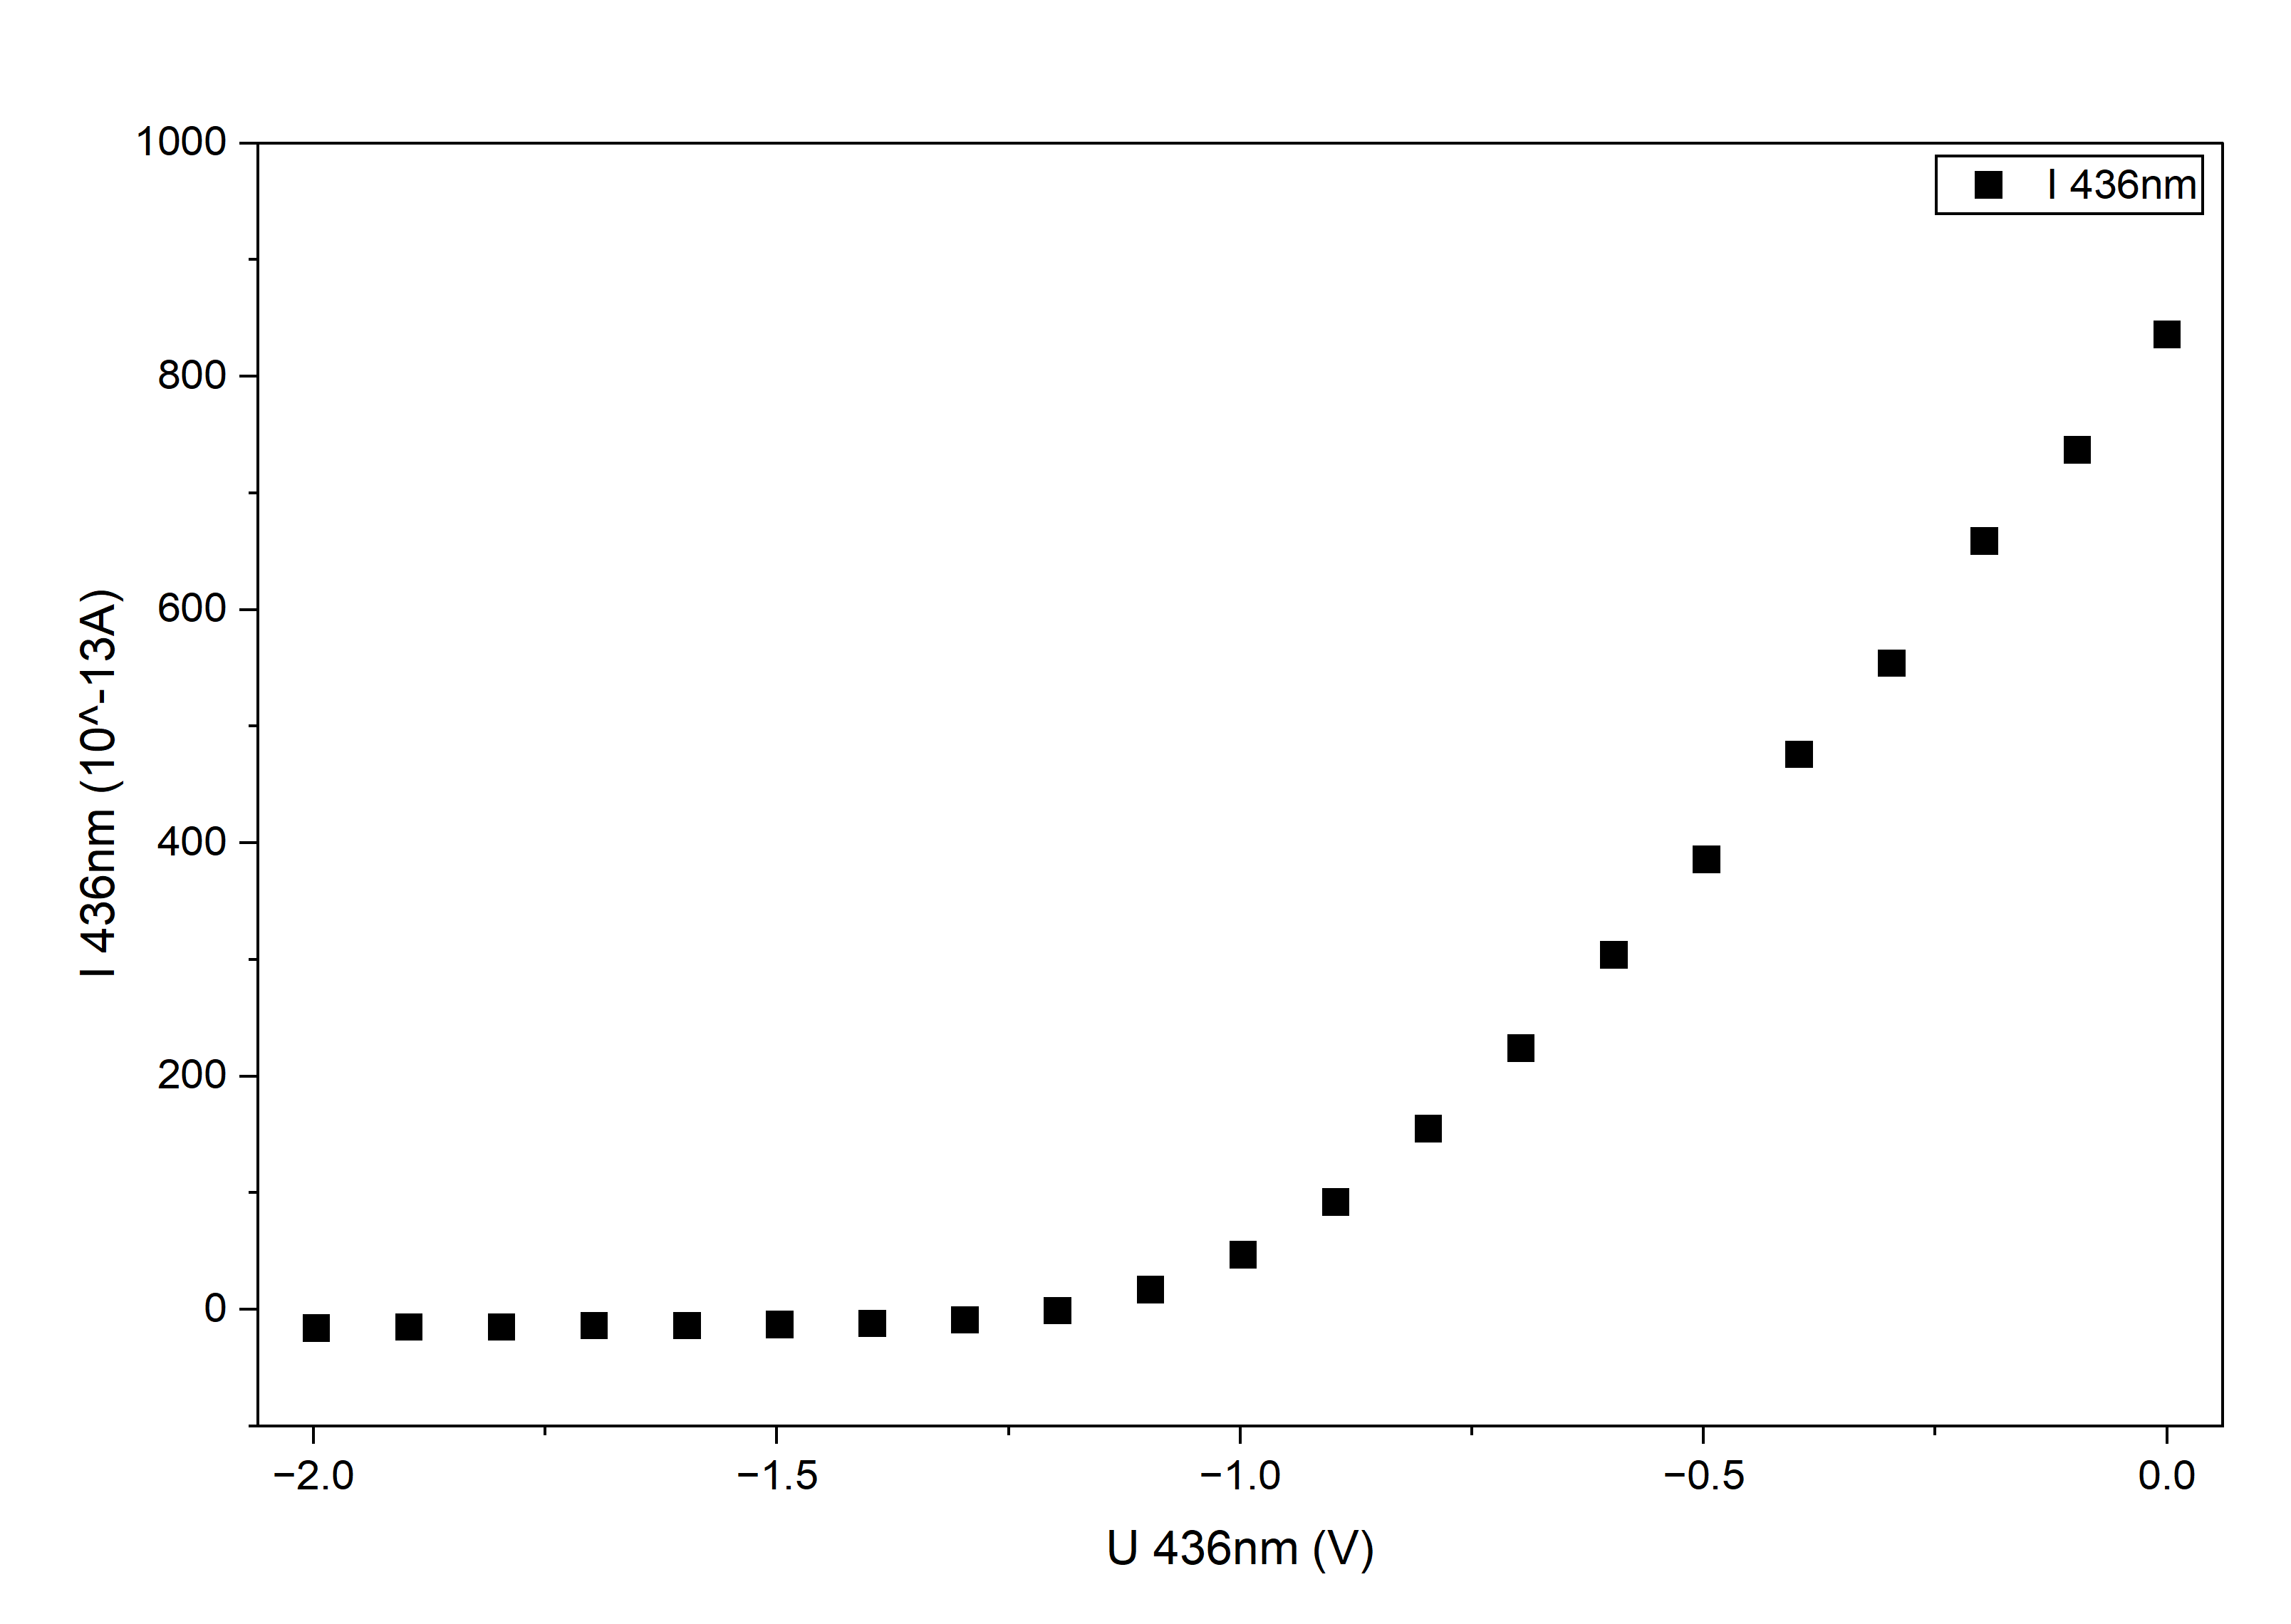
\includegraphics[width=0.9\textwidth]{436.png}
		\caption{436nm 波长光电管伏安特性曲线}
		\label{fig:436nm}
	\end{figure}\begin{figure}[H]
		\centering
		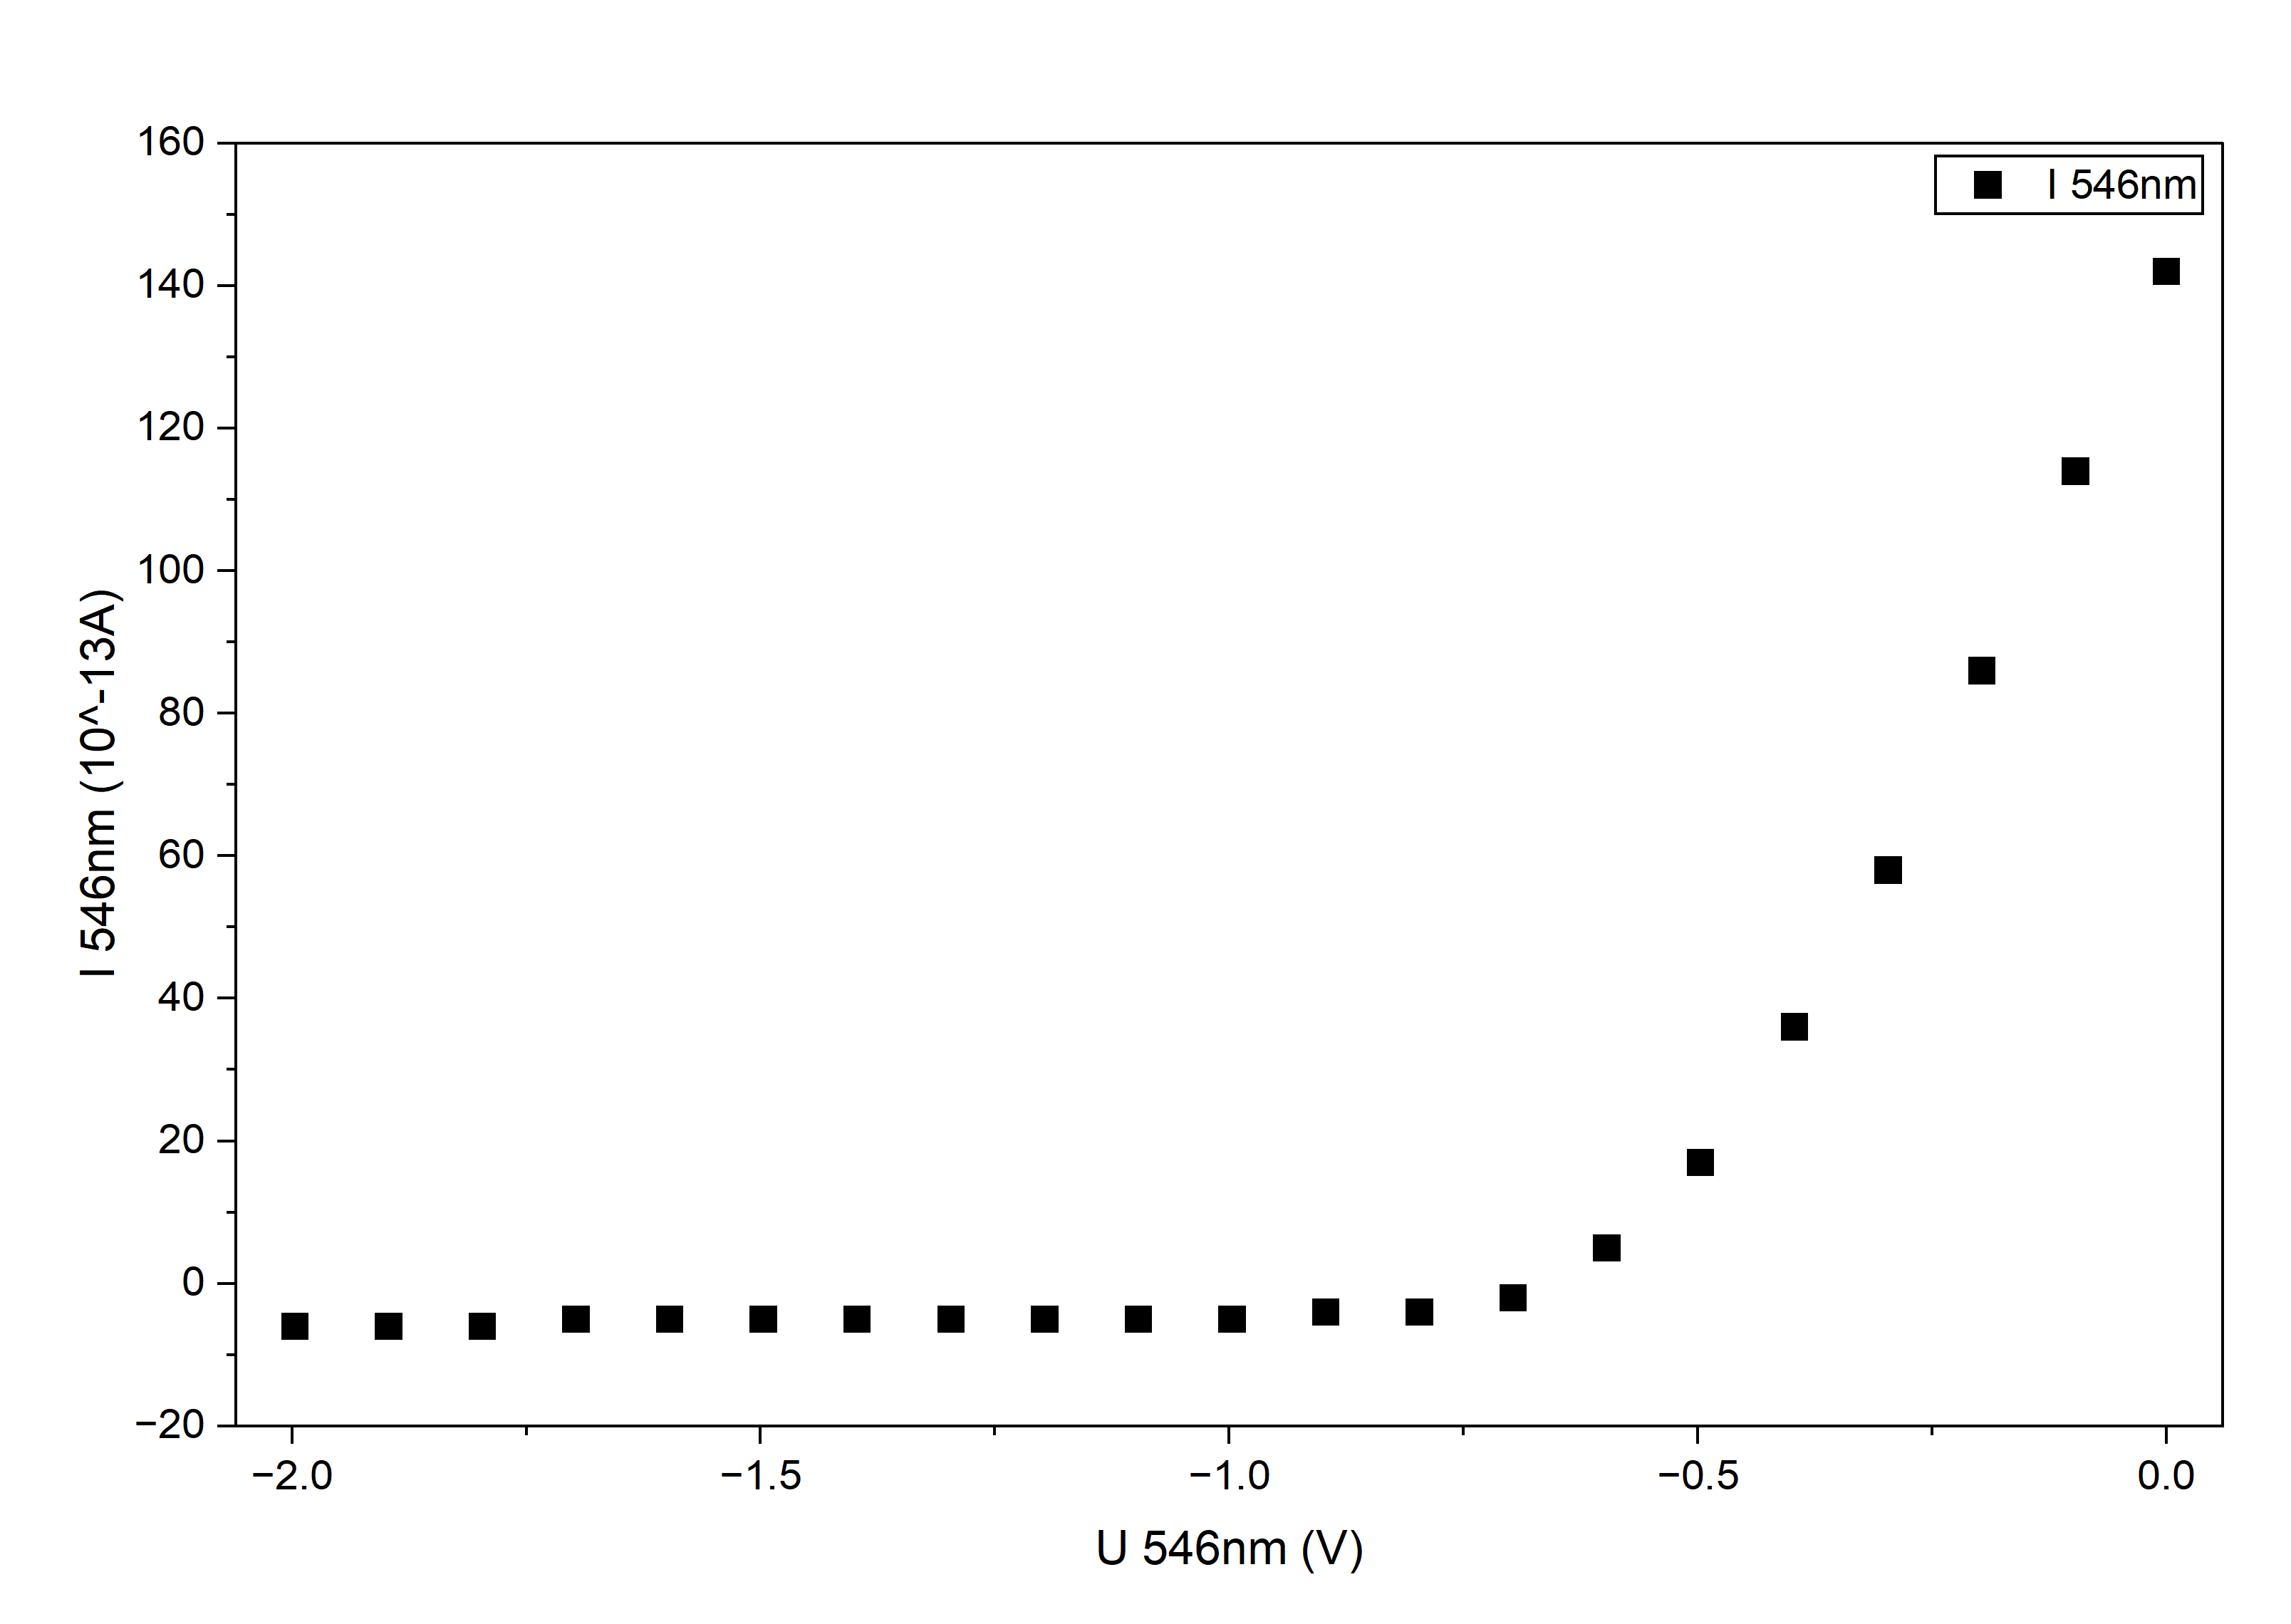
\includegraphics[width=0.9\textwidth]{546.png}
		\caption{546nm 波长光电管伏安特性曲线}
		\label{fig:546nm}
	\end{figure}\begin{figure}[H]
		\centering
		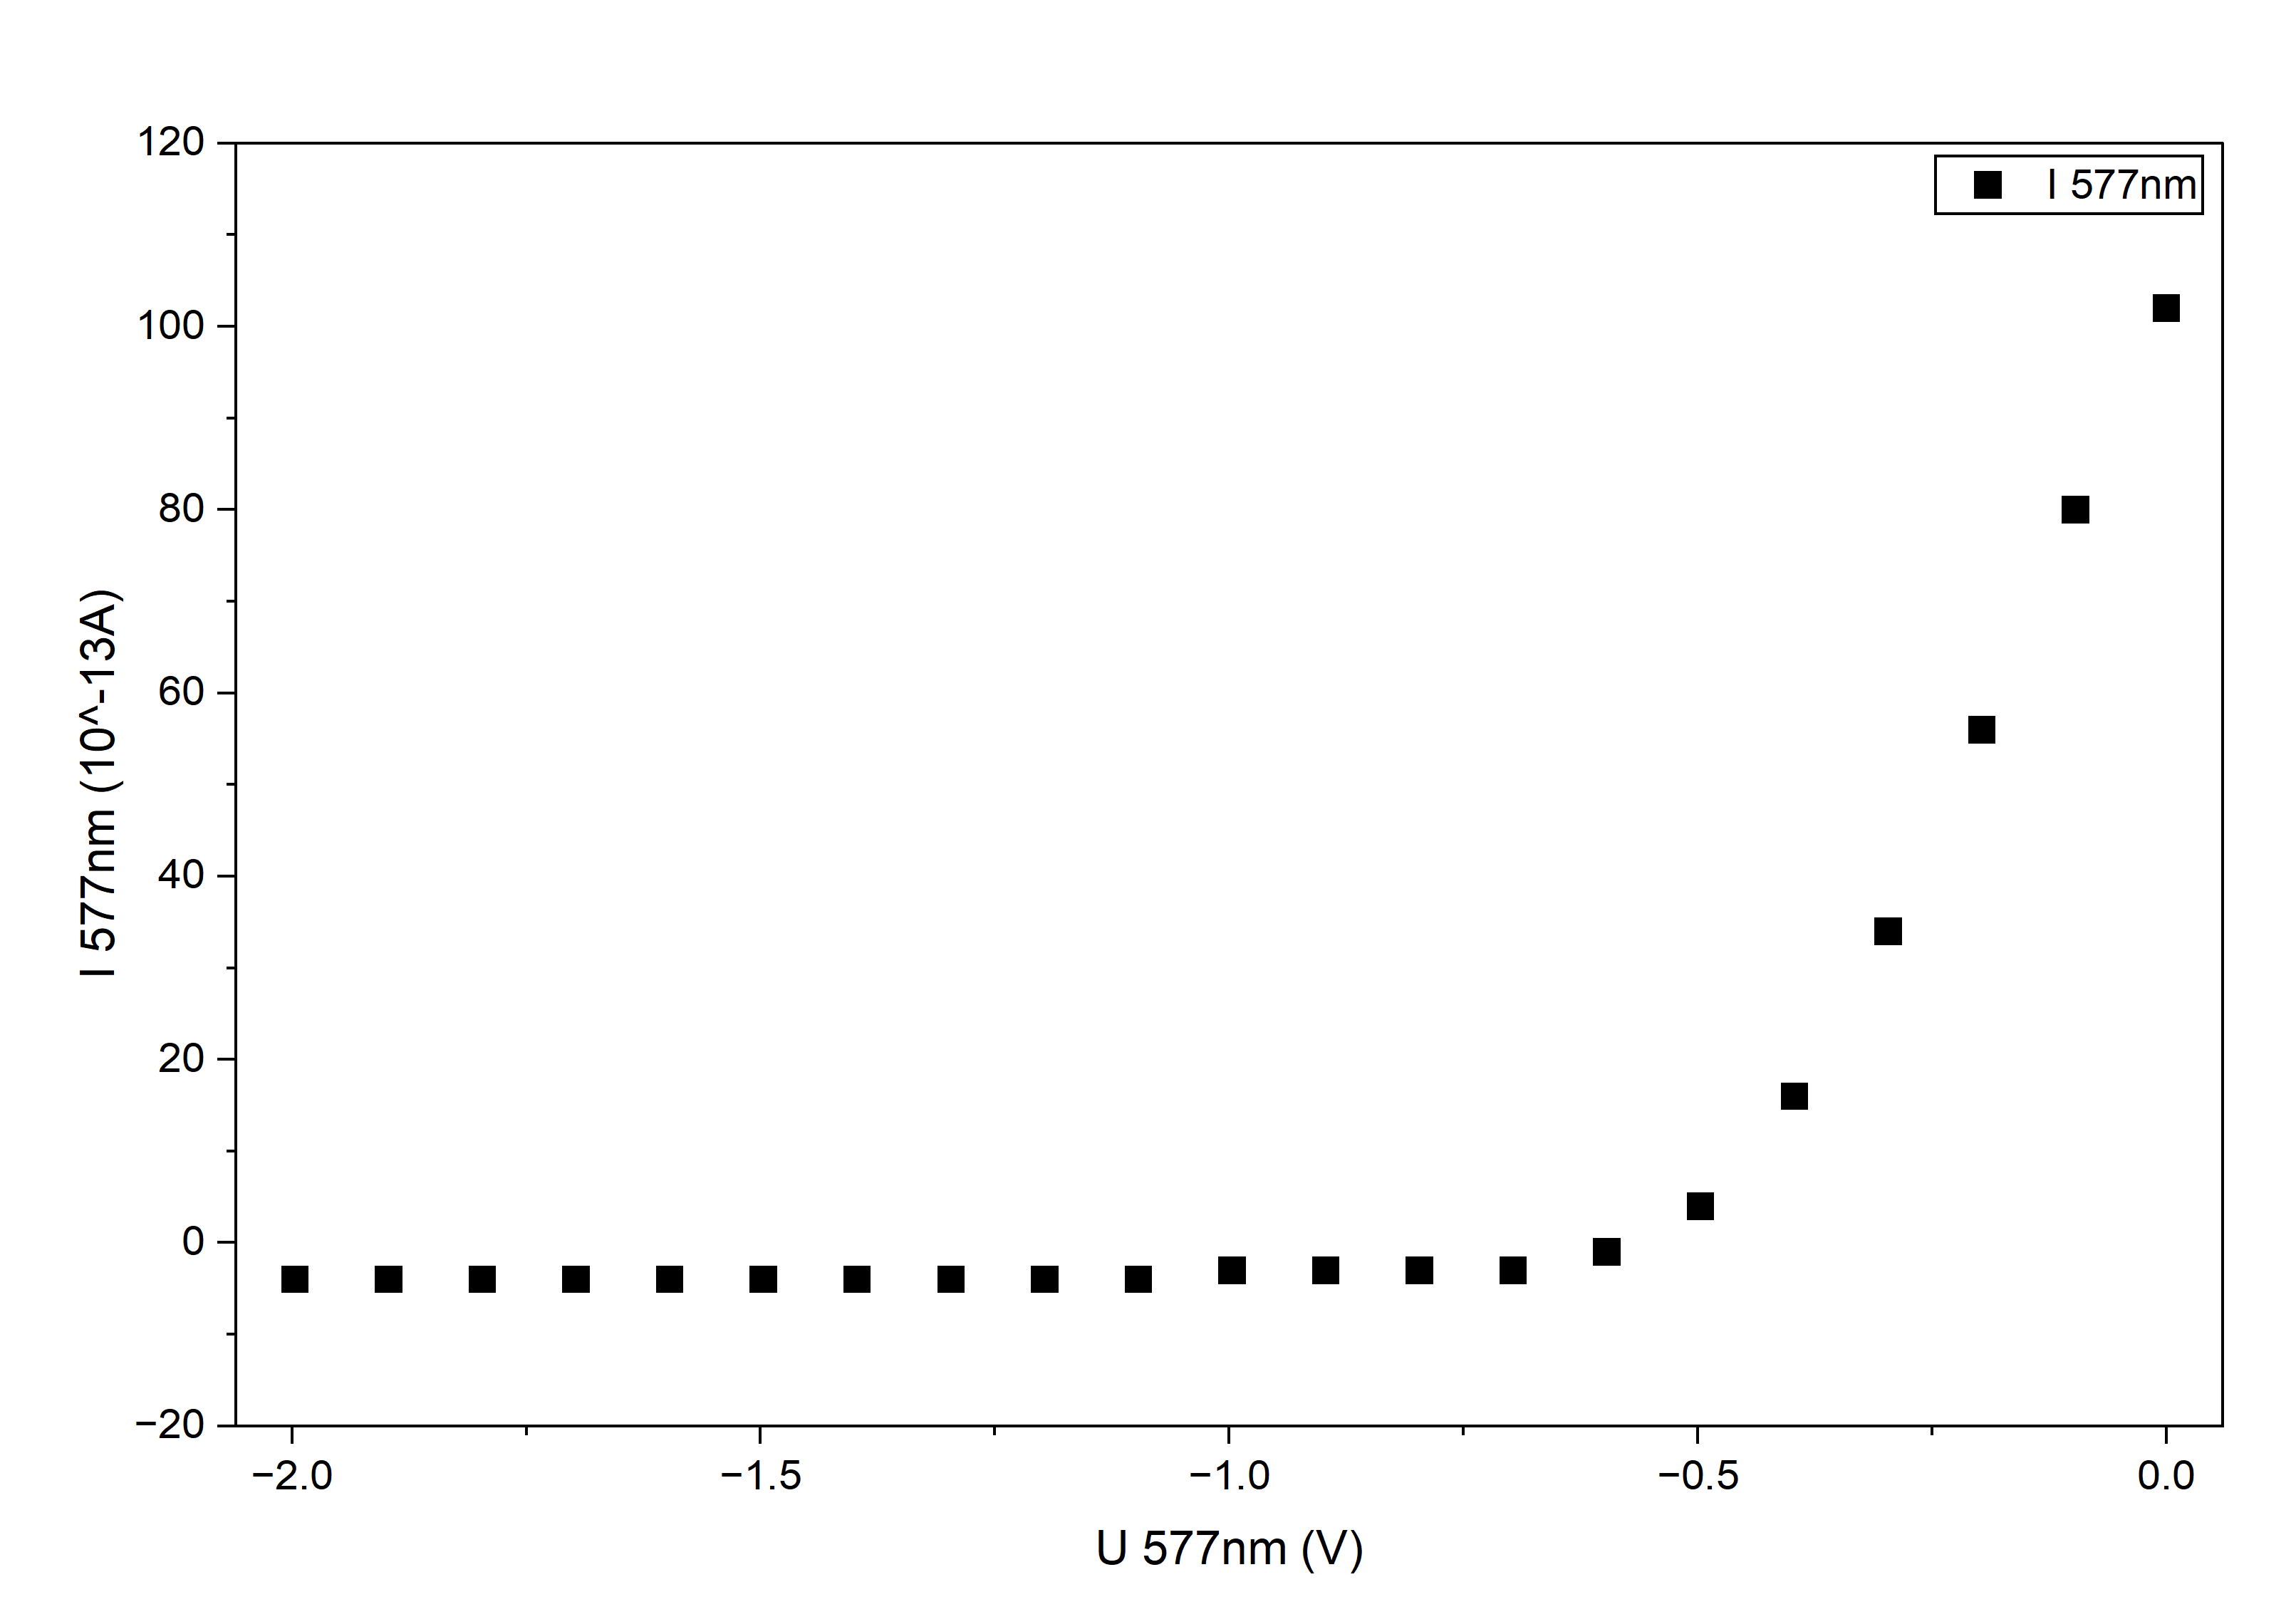
\includegraphics[width=0.9\textwidth]{577.png}
		\caption{577nm 波长光电管伏安特性曲线}
		\label{fig:577nm}
	\end{figure}

	根据伏安特性曲线，得到各波长对应遏止电压，如下表所示：
	\begin{table}[H]
		\centering
		\begin{tabular}{c c}
			\toprule
			波长 (nm) & 遏止电压 $U_a$ (V) \\
			\midrule
			365 & -1.797 \\
			405 & -1.398 \\
			436 & -1.199 \\
			546 & -0.697 \\
			577 & -0.596 \\
			\bottomrule
		\end{tabular}
		\caption{不同波长对应遏止电压}
		\label{tab:stopping_voltage}
	\end{table}
	
	\item \textbf{拟合遏止电压-频率曲线并计算各物理量}
	
	根据波长计算频率 $\nu = \frac{c}{\lambda}$，并作出遏止电压 $U_a$ 与频率 $\nu$ 的关系图像，进行线性拟合，得到下图：

	\begin{figure}[H]
		\centering
		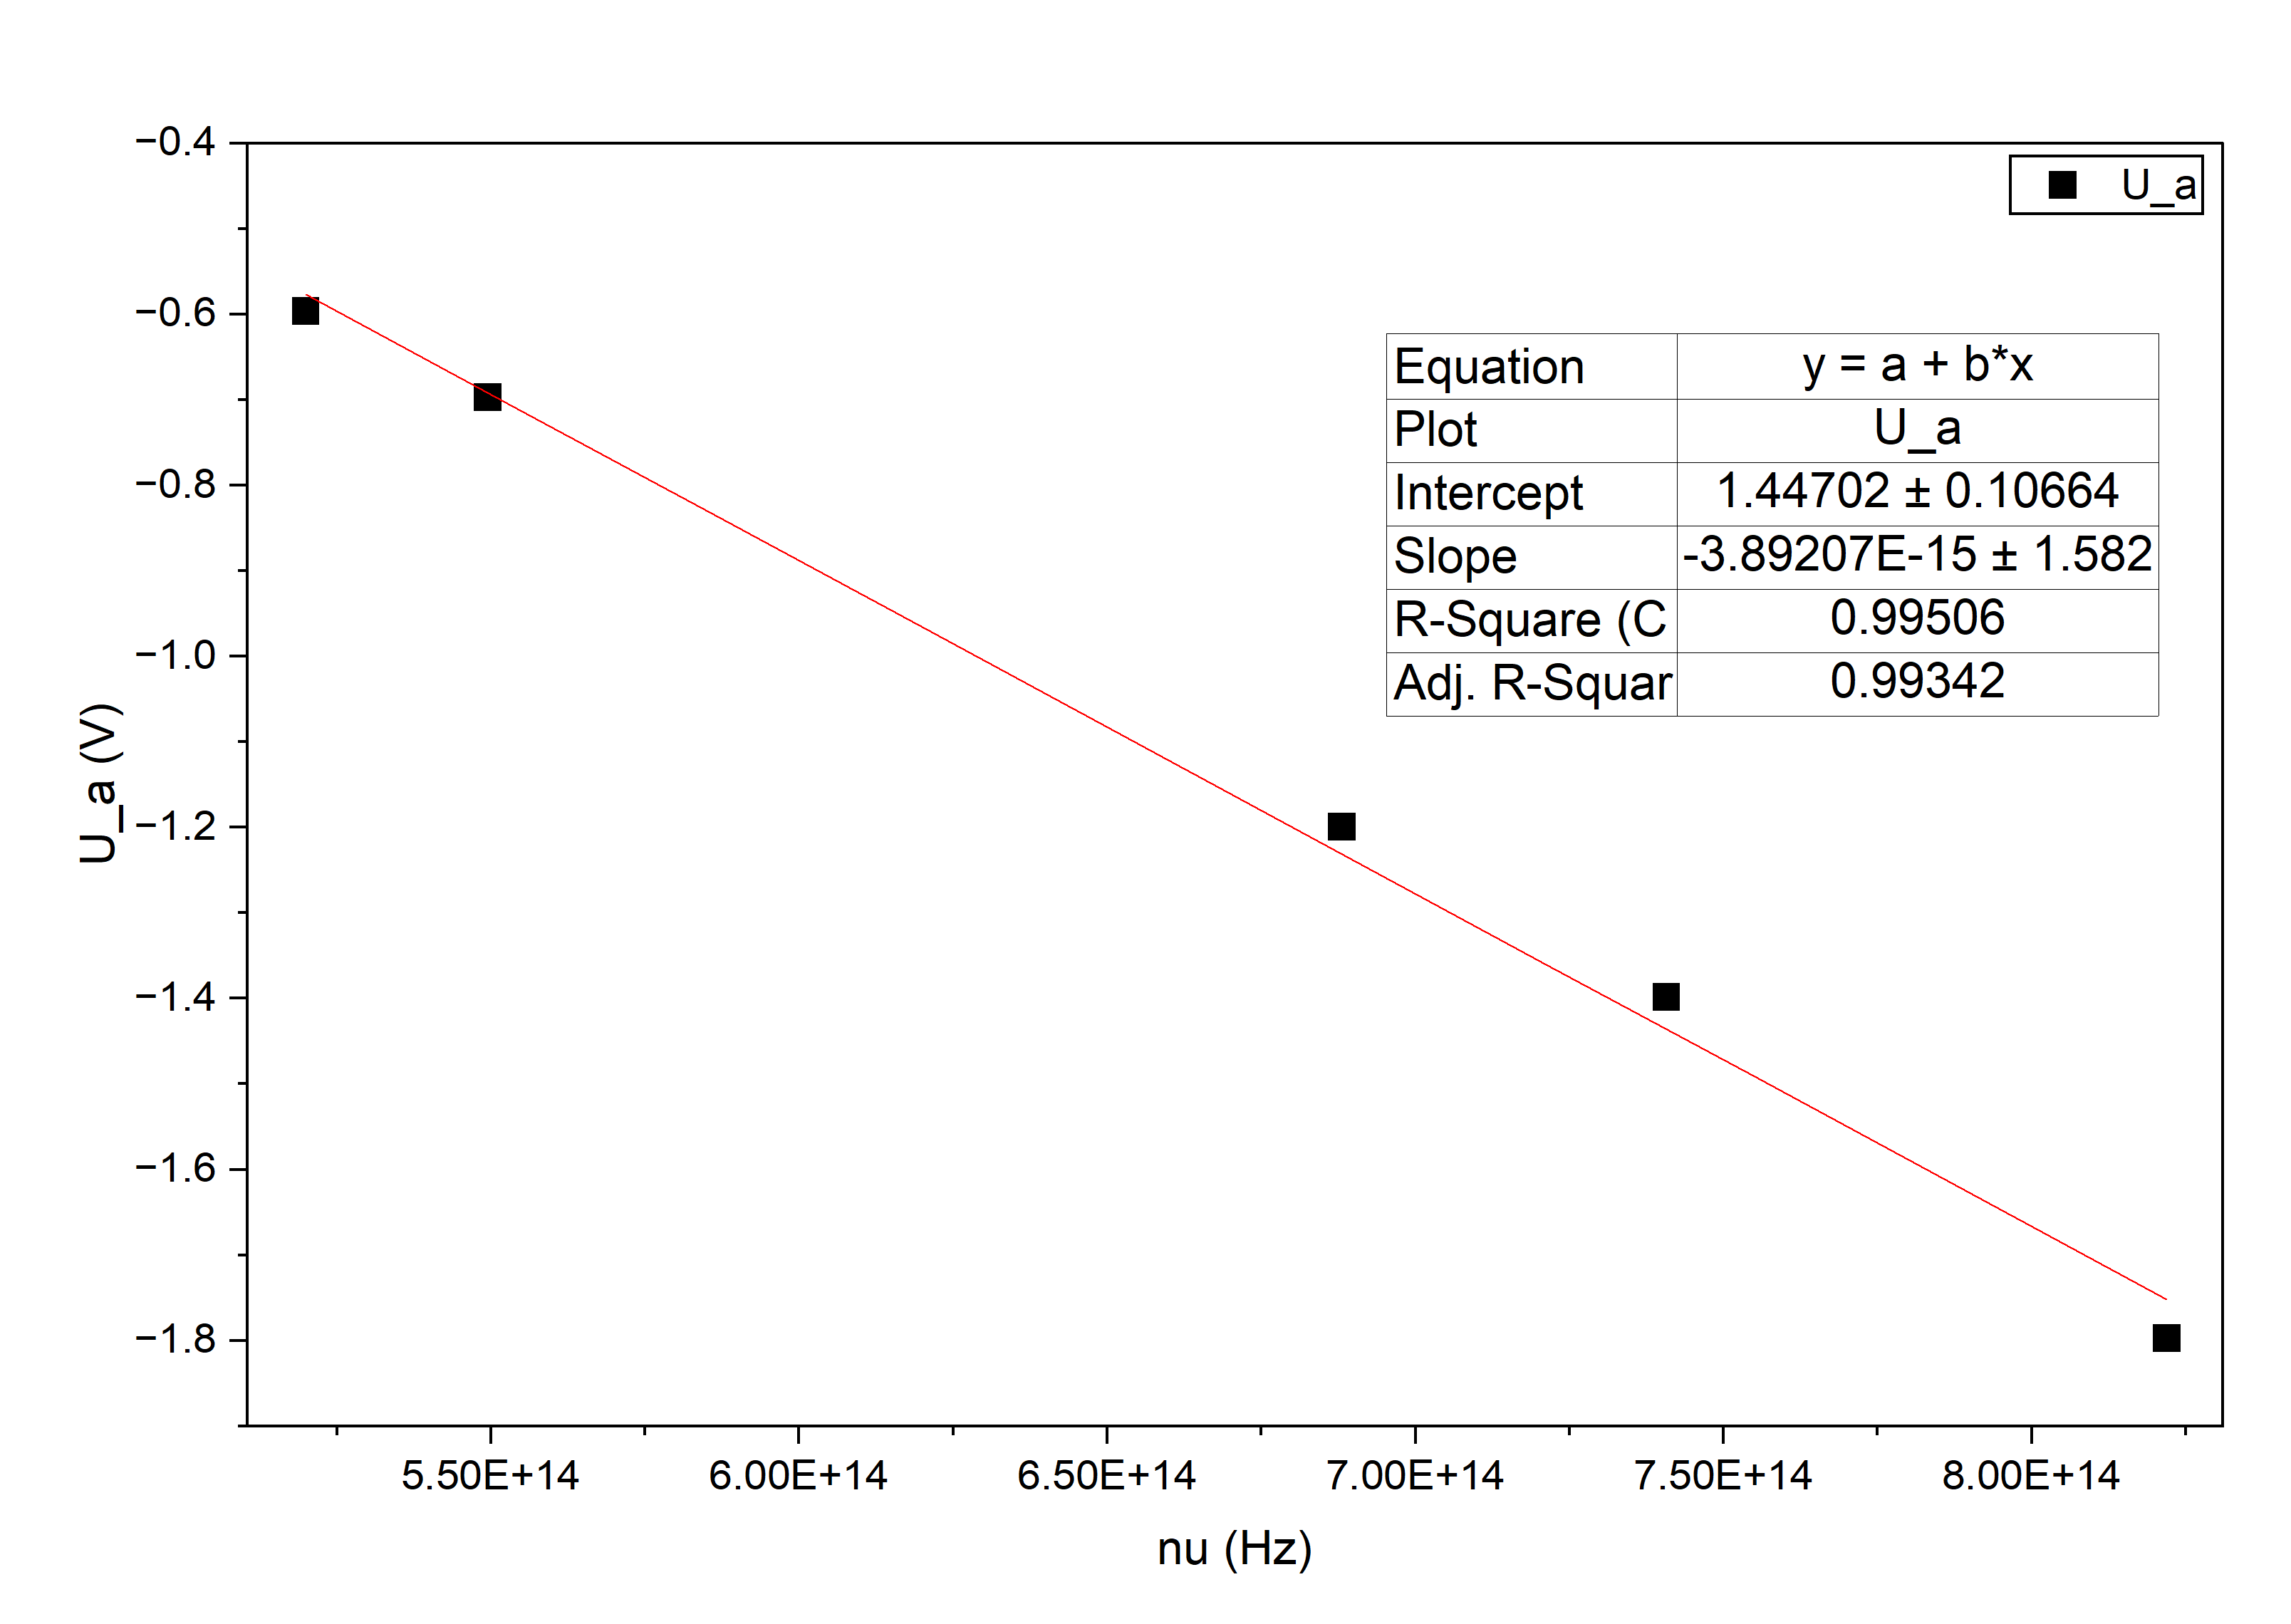
\includegraphics[width=1\textwidth]{3.png}
		\caption{遏止电压 $U_a$ 与频率 $\nu$ 关系图像}
		\label{fig:Ua_nu}
	\end{figure}

	拟合曲线斜率 $k = -3.89207\times 10^{-15}$，则普朗克常数
	$$h = k\cdot e = (-3.89207\times 10^{-15}) \times (-1.602 \times 10^{-19}) = 6.235 \times 10^{-34}\mathrm{J\cdot s}$$

	普朗克常数理论值 $h_0 = 6.626 \times 10^{-34}\mathrm{J\cdot s}$，则相对误差 
	
	$$\epsilon = \dfrac{|h-h_0|}{h_0} = \dfrac{|6.235 \times 10^{-34} - 6.626 \times 10^{-34}|}{6.626 \times 10^{-34}} = 0.059$$

	拟合曲线截距 $b = 1.44702$，则逸出功

	$$A = b \cdot e = 1.44702 \times 1.602 \times 10^{-19} = 2.318 \times 10^{-19} \mathrm{J}$$

	红限频率 $\nu_0 = \dfrac{A}{h} = \dfrac{2.318 \times 10^{-19}}{6.235 \times 10^{-34}} = 3.717 \times 10^{14} \mathrm{Hz}$。

	\end{enumerate}
	
	
	\section*{\textbf{八. 误差分析}}

	\begin{enumerate}
		\item 环境光与滤光片带宽导致入射光频率 $\nu$ 不精确；
		\item 热电子发射或杂散光引起暗电流等非光电流；
		\item 电压表、电流表的精度限制；
		\item 实验数据点分散或拟合点数不足导致线性拟合误差。
	\end{enumerate}

	
	\section*{\textbf{{九. 实验结论}}}

	本实验使用光电效应方法，测得普朗克常数 $h = 6.235 \times 10^{-34}$，逸出功 $A = 2.318 \times 10^{-19}$，红限频率 $\nu_0 = 3.717 \times 10^{14}$，其中普朗克常数相对误差为 $\epsilon = 0.059$。该实验验证了光电效应的基本原理。

\end{document}